\section{Impact Analysis}
An impact analysis serves the purpose of helping a developer understand the implications and impact of performing a refactor or introducing a feature into a software project. This is especially relevant, as the group consists of 5 total members, each refactoring their own feature, which could very quickly result in overlapping code changes, code constantly breaking and the end product becoming unstable.

To perform this impact analysis, we're making use of the program featureous and FeatureEntryPoint annotations to annotate parts of the program that is planned to be refactored. By doing this, we can gain a further understanding of the interconnectivity of the program and see how the features overlap code-wise.

The FeatureEntryPoints created for my feature are for the following methods and constructors.

\begin{itemize}
    \item OpenFileAction constructor
    \item actionPerformed in OpenFileAction.java
    \item openViewFromURI in OpenFileAction.java
    \item showDialog in OpenFileAction.java
    \item createDialog in OpenFileAction.java
\end{itemize}

Based on these FeatureEntryPoints, the generated report can be used to analyze the impact of the feature.

\subsection{Featureous Feature-Code Characterization}
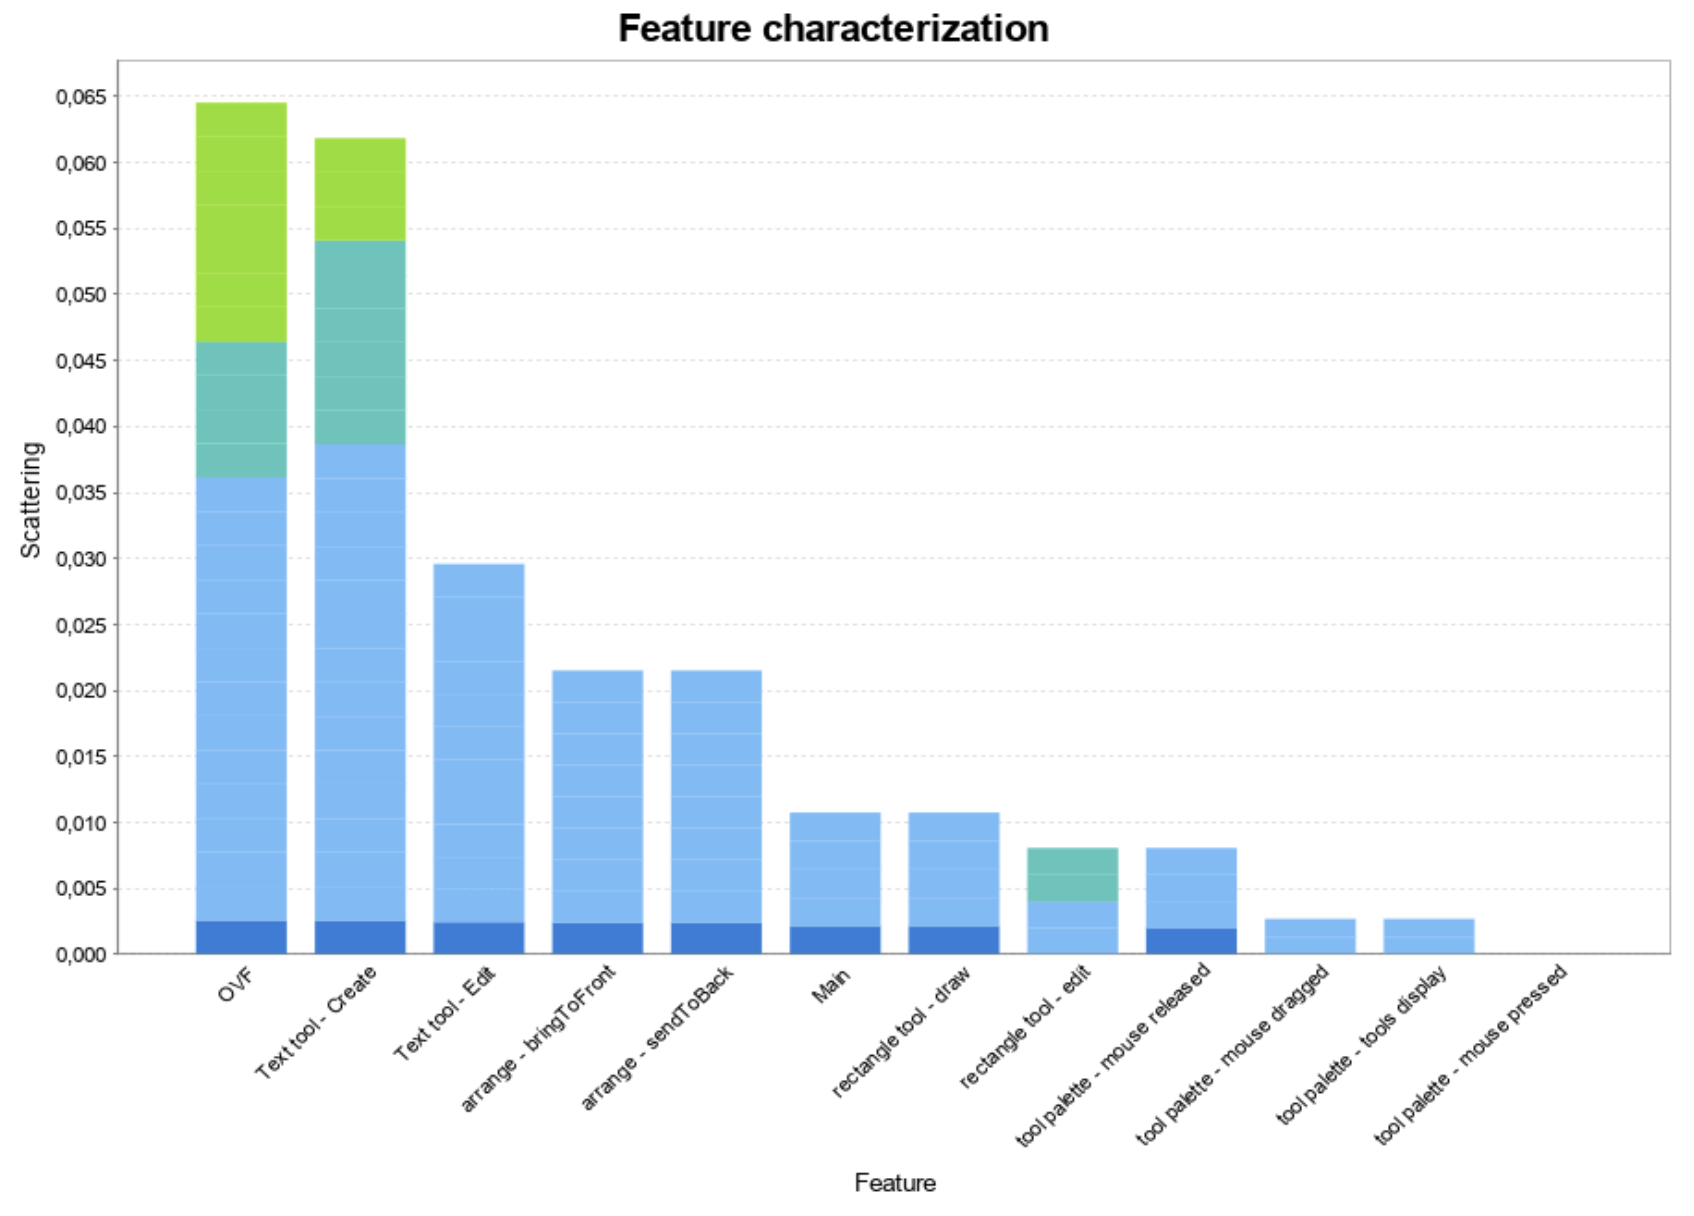
\includegraphics[width=\textwidth]{Images/featurecharacterization.png}
The above graph from featureous shows that my feature, here annotated as OVF, has a great deal of overlap with other features and is very scattered in the codebase. This means, that when refactoring, I need to be extra careful not to accidentally break other features, causing additional refactoring between me and another team member to be necessary.

\subsection{Feature Correlation Grid}
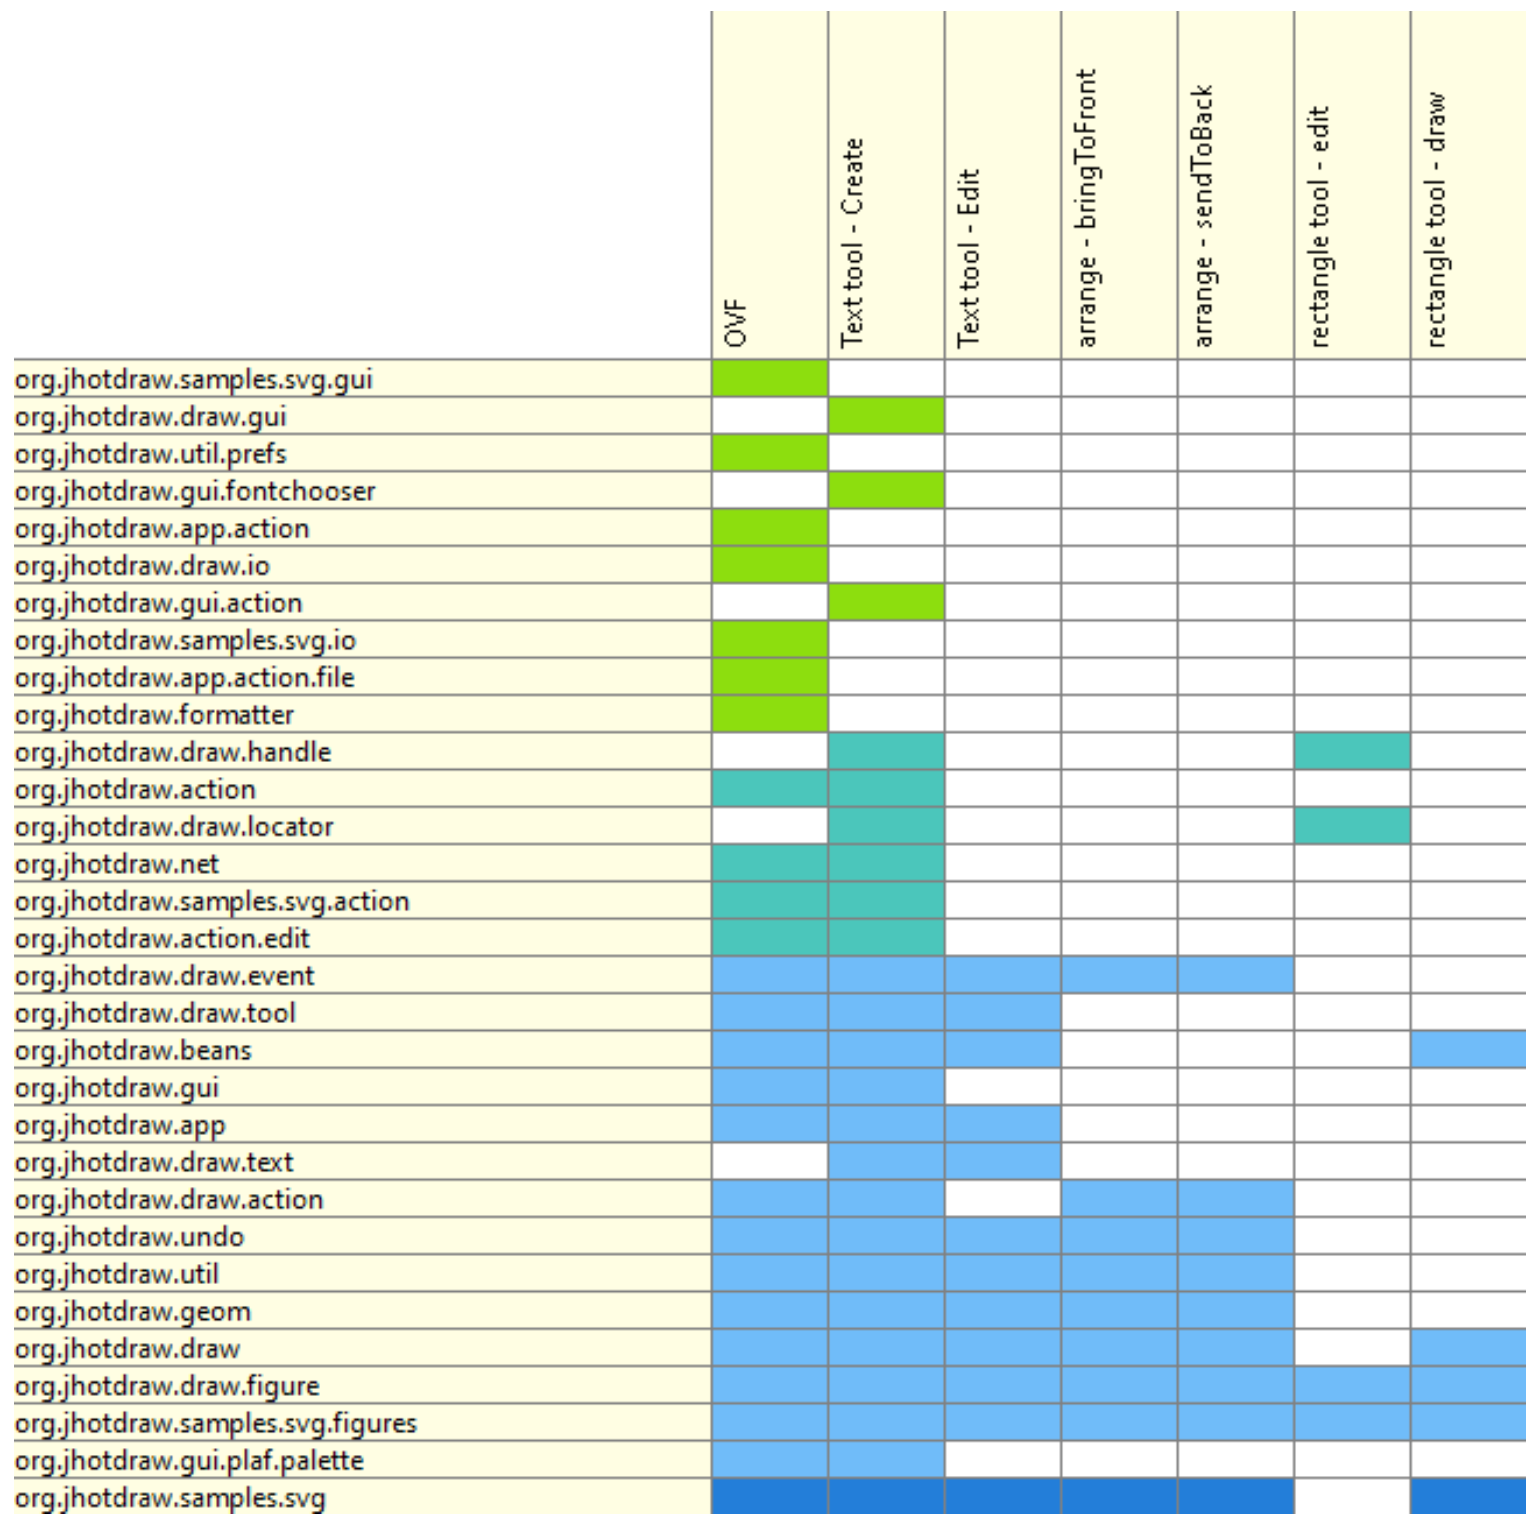
\includegraphics[width=\textwidth]{Images/featureousgrid.png}
\subsection{Feature Correlation Graph}
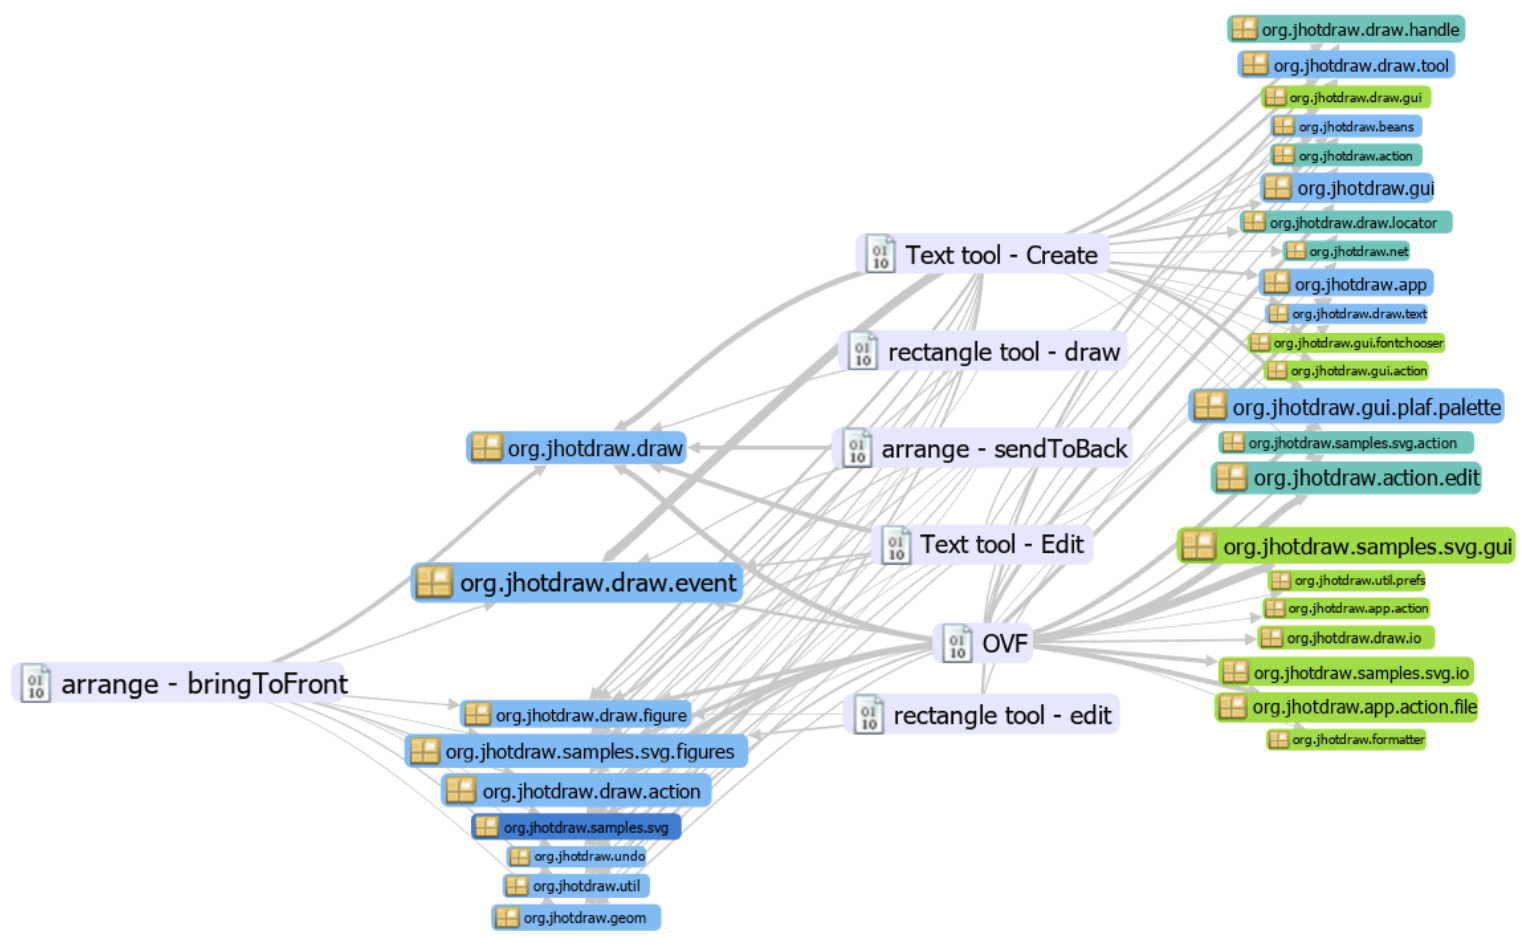
\includegraphics[width=\textwidth]{Images/featureousgraph.png}
Use Feature-code correlation graph and feature-code correlation grid to illustrate detailed investigations of the correspondences between source code units and related features to your change request.

Using table 2 list the packages and their number of classes that you visited after you located the concept. Write short comments explaining what you have learned about each package and how they contribute to your feature?
\subsection{Feature Relations Characterization}
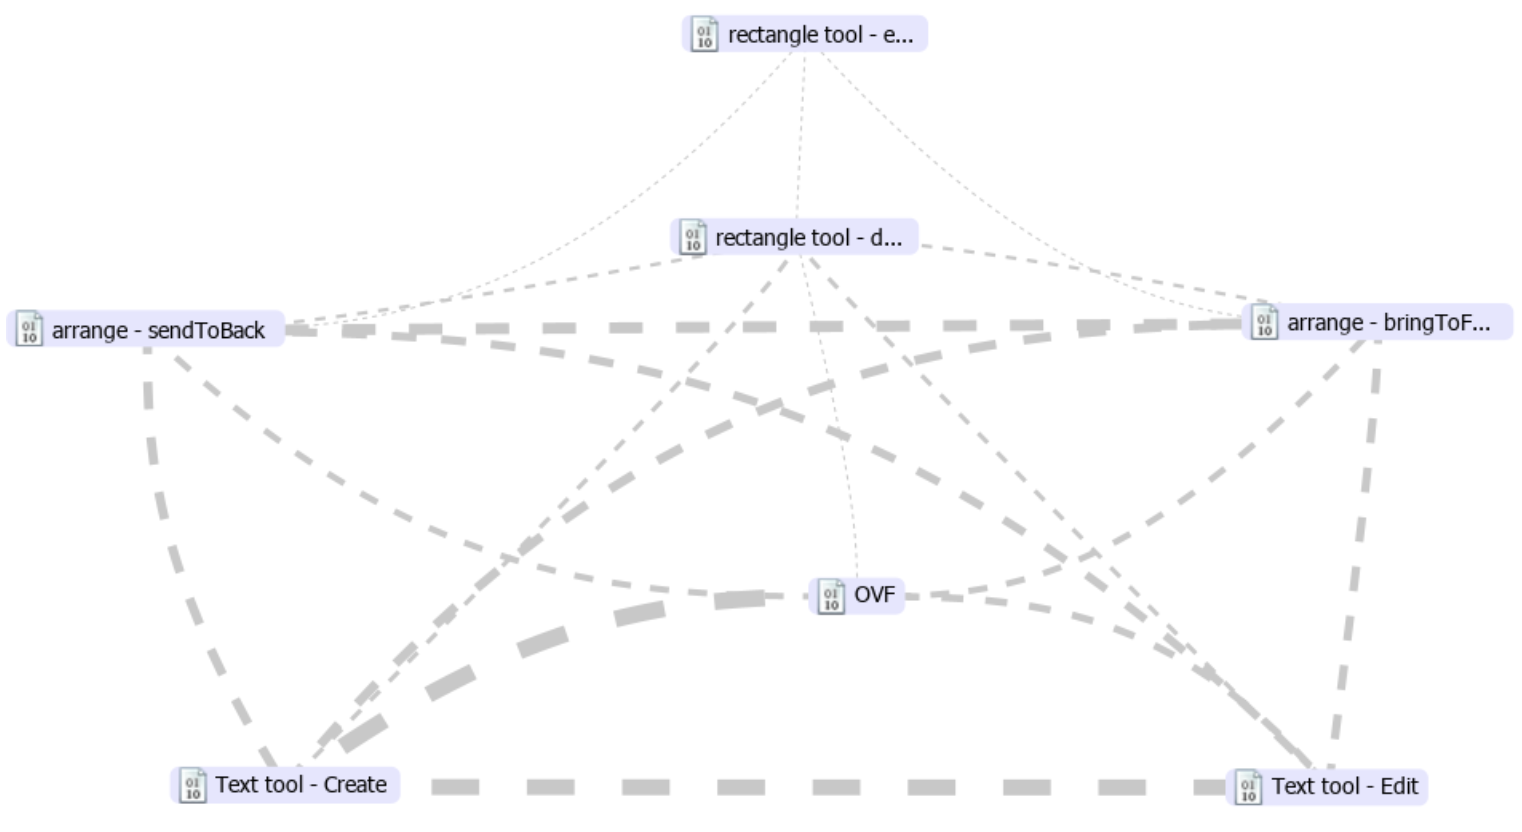
\includegraphics[width=\textwidth]{Images/featureousrelations.png}
Use Featureous Feature Relations Characterization view to relate your change request features to each other with respect to how they depend on the objects created by other features and how they exchange data by sharing these objects with one another.
\subsection{Dependency Analysis}

Show the features that my feature depends on

\subsection{Impact Analysis}
In the fourth column, mention if the class is related to the concept. Use one of the following terms:
\begin{itemize}
    \item Use “Unchanged” if the class has no relation to the concept but you have visited it.
    \item Use “Propagating” if you read the source code of the class and it guides you to the location of the concept, but you will not change it.
    \item Use “Changed” if the class will be changed.
\end{itemize}


\begin{longtblr}[caption = {The list of all the packages visited during impact analysis.}]{|l|l|l|l|}
    \hline
    \bf{Package name} & \bf{\# of classes} & \bf{Tool used} & \bf{Comments} \\
    \hline
    \bf{}             & \bf{}              & \bf{}          & \bf{}         \\
    \hline
    \bf{}             & \bf{}              & \bf{}          & \bf{}         \\
    \hline
    \bf{}             & \bf{}              & \bf{}          & \bf{}         \\
    \hline
    \bf{}             & \bf{}              & \bf{}          & \bf{}         \\
    \hline
\end{longtblr}
